\documentclass[UTF8]{article}

%--
\usepackage{ctex}
\usepackage[margin=1in]{geometry}
\usepackage{graphicx}


%--
\begin{document}
    
%--
{\flushleft \bf \Large 姓名:} 杨佩成

{\flushleft \bf \Large 学号:} MG1733079

{\flushleft \bf \Large 日期:} 2017.11.20


%=========================================================================
\section*{论文信息}
    
Burrows M. The Chubby lock service for loosely-coupled distributed systems[C]// Symposium on Operating Systems Design and Implementation. USENIX Association, 2006:335-350.


    
\section{概述}
	Chubby是一个面向松耦合分布式系统的锁服务,其主要目标是要解决分布式系统中的一致性问题,例如服务器中leader的选取。此外,Chubby还提供了少量的元数据存储服务。Chubby的设计目标主要包括高可靠性、高可用性和易理解的语义,吞吐量和存储能力被放在次要位置。Chubby假设要解决的一致性问题是基于异步消息通信模型的,这一模型可以描述现实中的大多数网络,允许通信过程中存在丢包、延迟和重传。Chubby使用了Paxos算法来解决系统中的一致性问题。    
%--
\section{设计}
	\subsection{基本原则}
	Chubby选择设计为锁服务而不是library主要是基于以下几点考虑:
\begin{itemize}
	\item
		开发人员在最初可能不会考虑系统的高可用性,但是随着系统的成熟和用户的增加,可用性越来越重		要,数据的复制和leader的选举就需要加入到设计中。锁服务可以方便的添加这些功能并且保持现有程序		的结构和通信模式。
	\item
		在广播服务结果时,需要Client读写一些小文件。这可以通过命名服务来实现,但是锁服务本身就可		以完成这个任务。
	\item
		程序员更加熟悉基于锁的接口。
	\item
		锁服务可以不需要基于Quorum做决定,这可以保证即使在客户系统的大多数成员没有启动时,客户系		统也可以做出正确的决定。
\end{itemize}

\indent Chubby中的锁是粗粒度的,粗粒度的锁可以持有几小时甚至几天。相比于细粒度的锁,粗粒度的锁对锁服务器的负载要少得多。但是粗粒度锁在不同客户端切换时会需要更多的操作,来保证服务器失效时能正常恢复。而细粒度的锁即使是短暂的失效也会导致许多客户端停止。Chubby中选择粗粒度锁提高了系统的可用性,放宽了一些性能上的要求。但是在Chubby中,用户可以根据自己应用方便地实现自己的细粒度锁。
	\subsection{系统结构}

\begin{figure}[htbp]
\centering
\small
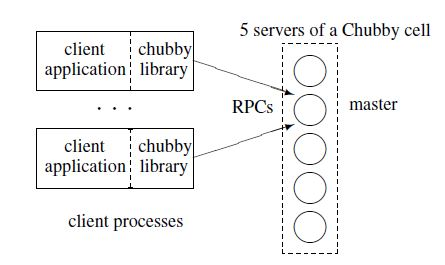
\includegraphics{1.JPG}
\caption{System structure}
\end{figure}
	Chubby主要由服务端和客户端两部分组成,二者通过RPC进行通信。每个客户端的应用都有一个Chubby library,客户端通过Chubby library与服务端交互,如Figure 1所示。
	
	每个Chubby cell都由一组服务器组成(一般是五台),每台服务器都作为一个副本,使用副本主要是为了防止单个节点的失效或者网络的异常,以达到高可靠性和高可用性的目标。同一个cell里的副本服务器维护的是同一个数据库的副本,只有master服务器可以处理数据库的读写请求,其他服务器只是通过一致性协议复制master里的更新。副本服务器通过分布式系统的一致性协议来选举master,master必须获得大多数副本服务器的投票并且在一个master租期中不会选出新的master。master的租期可以一直被延长,只要master能够一直赢得大多数服务器的选票。

	客户端通过向所有服务器发送master定位请求来找到master的位置,非master服务器收到请求会返回master的位置。当客户端知道了master的位置后,所有的请求就直接发送给master。写请求会通过一致性协议传播给其它服务器,当写操作在大多数服务器上完成后请求才会被答复。读请求只需要master就可以完成。

\subsection{实现}
	Chubby本质上是一个分布式的、存储了大量小文件的文件系统,Chubby中的锁就是文件。用户通过操作文件,获取共享锁或独占锁。Chubby使用了一种类似于UNIX的文件系统,并做了一些针对分布式系统的优化:不提供文件的移动操作,不记录目录修改时间,不使用基于路径的权限管理。使用这种文件系统,简化了系统开发的工作量,并且也降低了Chubby用户的学习成本。

	在Chubby中文件和目录统称为node,每个node名在Chubby cell中都是唯一的。每个node都有很多元数据,包括存储了读、写、修改权限列表(ACL)的三个文件名以及文件版本号和校验和等元数据。Chubby通过类似于UNIX的Handle对node进行访问。

	Chubby中的每个node都可以作为一个读写锁,在写模式下客户端唯一的持有锁,在读模式下多个客户端可以共享锁。Chubby中实现的是Advisory lock而不是Mandatory lock,这么选择主要从以下几点考虑:Chubby锁通常是为了保护其它服务所使用的资源,若使用Mandatory lock会需要开发者对这些服务做更多的修改;使用Advisory lock能够访问加锁Node的数据,方便数据共享和调试。
	
	在分布式系统中锁是非常复杂的,因为通信的不确定和进程的失效,这会导致服务器处理的数据是乱序的。这种问题通常通过virtual time和virtual synchrony等算法解决。但是在现有的复杂系统上对所有的交互都引入序列号,代价是很高的,所以Chubby只对涉及到使用锁的交互操作引入序列号。锁的持有者可以请求一个sequencer,它包括了锁的名字、模式和锁的生成序号。当客户端需要执行被锁保护的操作时,客户端要将sequencer传给服务器。如果服务器判定sequencer无效,就会拒绝客户端的请求。

	尽管sequencer很容易使用,但是相关的重要协议发展得很慢。因此Chubby还提供了一种不完美但是能够在不支持sequencer场景下使用的算法。当客户端正常释放锁时,该锁可以被立即获取;但是如果因为客户端失效而锁被释放,锁服务器会在一段时间内拒绝其他客户端的锁请求。
	
	为了减少客户端与服务器之间的通信量,Chubby的客户端会缓存部分文件数据和节点的元数据。当缓存的数据要被修改时,修改的操作会被阻塞。同时master给缓存了这些数据的客户端发送失效信息,客户端收到失效信息后清空失效数据的缓存并回复。master在收到客户端回复的信息后才会真正执行修改操作。
	


	





\end{document}

